After defining the business goals and the goals of data mining in the Business Understanding phase, the next crucial step in the CRISP-DM process is Data Understanding.
This phase involves collecting the initial dataset, examining its structure, and verifying data quality.
The primary goal is to become familiar with the dataset, identify potential quality issues, and extract early insights.

\begin{figure}[H]
    \centering
    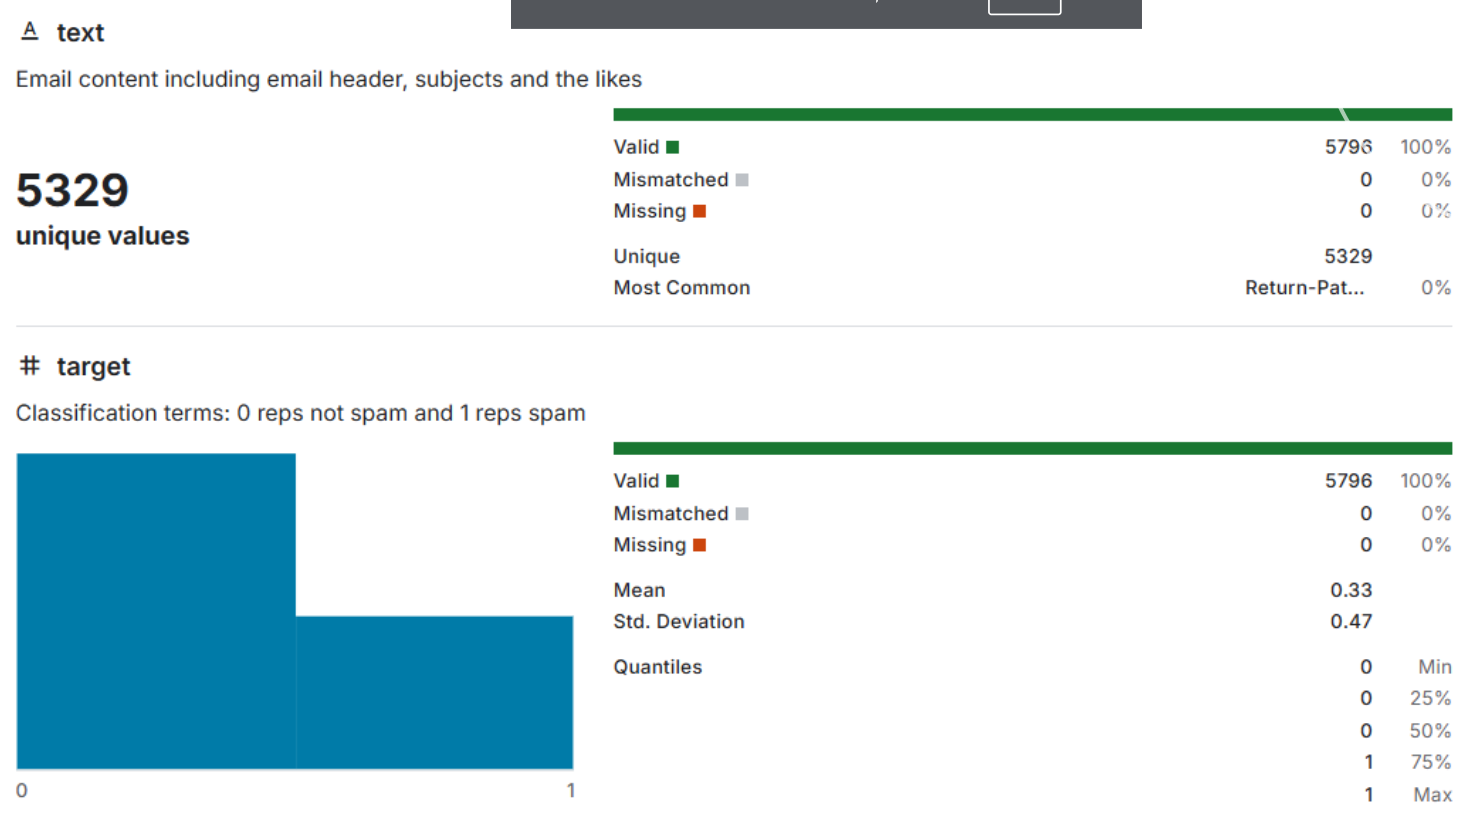
\includegraphics[width=\linewidth]{images/dataset_information}
    \caption{Dataset Information}
    \label{fig:dataset_information}
\end{figure}

In this image, we can see that out of all 5679 text values which included email headers, subjects and the likes, 5329 of them are unique values.
From this information, we can learn that the dataset has a large variety of values, and no duplicates are missing values that may impact the quality of the dataset significantly in any way.

Various NLP techniques were applied to explore the email content:

\subsection{Word Cloud}
\label{subsec:word-cloud}
Revealed high-frequency terms like number, url, date, mail, list, get, time, system, use, and HTML-related terms
(font, nbsp, td, tr).
The prevalence of number and url might indicate preprocessing/anonymization or simply be features of the emails.
HTML terms suggest formatted emails are common.

\begin{figure}[H]
    \centering
    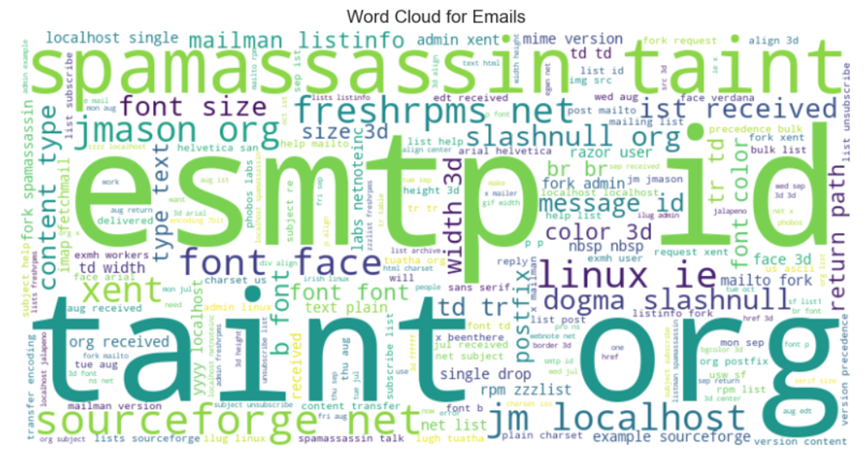
\includegraphics[width=\linewidth]{images/word_cloud}
    \caption{All emails in the form of Word Cloud}
    \label{fig:word_cloud}
\end{figure}

\smallskip
Prominent Keywords:

\begin{itemize}
    \item taint, spamassassin, esmtp, org, id, localhost, net, sourceforge: These are the largest and boldest words,indicating they are the most frequent and important terms within the analyzed email data.
    \item The rest of the word cloud: These words are smaller but still noticeable,suggesting they also play a significant role in the email context.
\end{itemize}

Possible Suggested Topics:

\begin{itemize}
    \item Spam Filtering: The presence of ``spamassassin'' and ``taint'' (often associated with marking suspicious emails) suggests a significant topic might be the identification and handling of spam.
    \item Mailing List Management: Words like ``list'',``listinfo'', ``mailman'', and ``mailing'' hint at discussions related to managing and interacting with email lists.
    \item Technical Email Information: Terms such as ``smtp'' (Simple Mail Transfer Protocol), ``mime'' (Multipurpose Internet Mail Extensions), ``version'',``id'', ``localhost'', and ``net'' indicate potential discussions about the technical aspects of email.
    \item Formatting and Display: Words like ``font'',``size'', ``face'', ``text'', and ``color'' might relate to how emails are displayed and formatted.
    \item Source and Path: ``sourceforge'' (an open-source software repository), ``received'', and ``path'' could be related to tracking the origin and route of emails.
    \item Related Systems and Software: ``linux'', ``xent'', and ``rpm'' might be the names of operating systems or software mentioned within the email context.
\end{itemize}

\subsection{Word Frequency (Top 10)}
\label{subsec:word-frequency}
After removing basic English stopwords and non-alphabetic tokens, the bar chart confirmed the dominance of words like number, url, mail, date, list, get.
Their persistence highlights their potential importance or noise factor.

\begin{figure}[H]
    \centering
    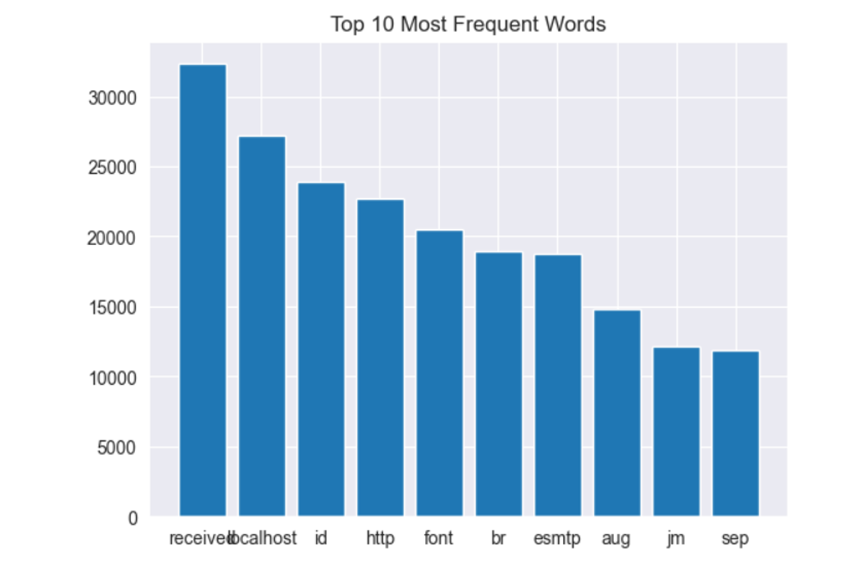
\includegraphics[width=\linewidth]{images/frequent_words}
    \caption{Bar Chart for 10 Most Frequent Words}
    \label{fig:frequent_words}
\end{figure}

The most frequent word is ``received'', with a significantly higher count (over 30,000) compared to the other top words.
This suggests that the word ``received'' appears very often in the analyzed text data after the filtering.

The following most frequent words, in descending order, are ``localhost'', ``id'', ``http'', ``font'', ``br'', ``esmtp'', ``aug'', ``jm'', and ``sep''.
These words have frequencies ranging from approximately 11,000 to 27,000.

The nature of the top words suggests the analyzed text data might be related to email headers or technical logs.
Words like ``received'', ``localhost'', ``id'', ``http'', and ``esmtp'' are commonly found in email metadata.
``aug'' and ``sep'' likely refer to month abbreviations.
``font'' and ``br'' could appear in the content or formatting information.

The code successfully identifies and counts the occurrences of words after applying basic text cleaning.
The use of nltk.word\_tokenize splits the text into individual words, .lower() converts them to lowercase for consistent counting, and the list comprehension filters out non-alphabetic tokens and common English stop words.

The Counter object efficiently calculates word frequencies, and most\_common(10) retrieves the top 10 most frequent words and their counts.
This data is then used to generate the bar chart using matplotlib.pyplot.

The visualization clearly shows the relative frequency of the top 10 words.
The height of each bar directly corresponds to the number of times that word appears in the processed text.


\subsection{Email Length Distribution}
\label{subsec:email-length-distribution}
The histogram showed a right-skewed distribution.
Most emails are short (under 500 words), but a long tail indicates the presence of very long outlier emails, adding diversity to the dataset structure.
Length could be a potential feature.

This code calculates how many words are in each email and then creates a bar chart (histogram) to show how many emails fall into different length categories (e.g., 0–500 words, 500–1000 words, etc.). It helps visualize the typical length of emails in our dataset.

\begin{figure}[H]
    \centering
    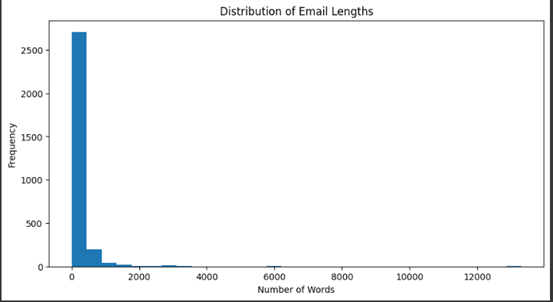
\includegraphics[width=\linewidth]{images/email_length_distribution}
    \caption{Bar Chart for Email Length Distribution}
    \label{fig:email_length_distribution}
\end{figure}

Distribution Shape:
\begin{itemize}
    \item Right-skewed: The majority of the bars are concentrated on the left side of the histogram, indicating that most emails are short in length.
    \item High Peak on the Left: The first bar (near zero words) has a significantly higher height than the other bars,showing a large number of very short emails.
    \item Long Tail to the Right: The bars gradually decrease towards the right, but there are still some emails with considerable length, extending to several thousand words.
\end{itemize}



\subsection{Common N-grams (Trigrams)}
\label{subsec:common-n-grams}
Analysis of the top 10 trigrams showed patterns like ``wed number aug'', ``number aug number'', ``date number number'', suggesting frequent date/number sequences or mailing list headers (list listinfo mail).
These patterns might help identify specific email types.

\begin{figure}[H]
    \centering
    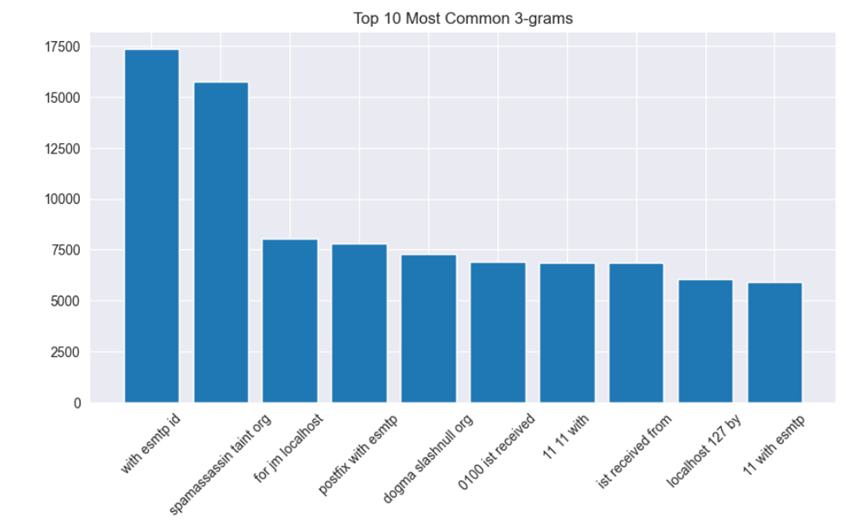
\includegraphics[width=\linewidth]{images/common_tri_grams}
    \caption{Bar Chart for 10 Most Common Trigrams}
    \label{fig:common_tri_grams}
\end{figure}

Observations:
\begin{itemize}
    \item The trigram ``with esmtp id'' is the most frequent, appearing significantly more often than the others.
    \item The trigram ``spamassassin taint org'' is the second most frequent.
    \item The remaining trigrams have lower and relatively similar frequencies.
    \item The trigrams suggest that the email data contains technical information, likely related to email headers and processing (``esmtp'', ``localhost'', ``received'') and spam filtering (``spamassassin'', ``taint'').
\end{itemize}

Potential Meaning:
\begin{itemize}
    \item The most frequent trigrams indicate the common occurrence of information related to email headers and the email transmission process.
    Phrases like ``with esmtp id'', ``postfix with esmtp'', ``ist received'', ``received from'', and ``localhost 127 by'' all pertain to how emails are sent and received.
    \item The presence of ``spamassassin taint org'' suggests that spam filtering activity is a significant aspect of this dataset.
    \item Other trigrams like ``for jm local/host'', ``dogma slashnull org'', ``0100 ist received'', ``11 11 with'', and ``11 with esmtp'' might relate to specific systems, software, or characteristic data formats within the context of this dataset.
\end{itemize}

Conclusion:

This chart reveals that information related to email processing and headers, as well as spam filtering activities, are prominent features in the analyzed text dataset.
The other trigrams may provide further insights into specific systems or formats relevant to this data.

\subsection{POS Tag Frequency}
\label{subsec:pos-tag-frequency}
The distribution of Part-of-Speech tags (NN, NNP, NNS, VB variants, JJ, IN being most frequent) confirmed that the email text follows typical English grammatical structures.

\begin{figure}[H]
    \centering
    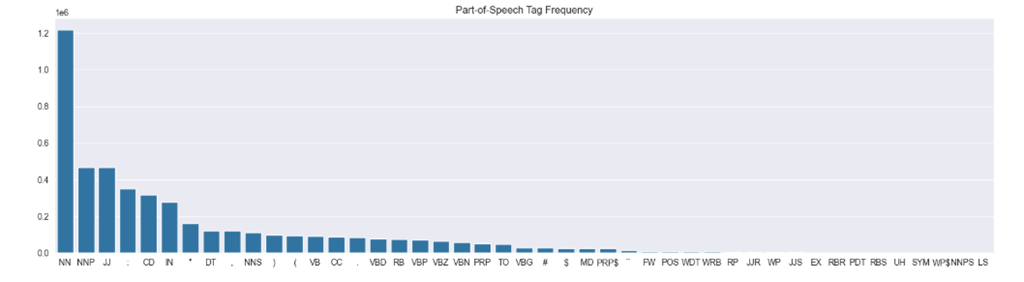
\includegraphics[width=\linewidth]{images/pos-tag-frequency}
    \caption{Bar Chart for POS Tag Frequency}
    \label{fig:pos-tag-frequency}
\end{figure}

Observations:
\begin{itemize}
    \item Nouns are highly frequent: The tags ``NN'' (singular nouns) and ``NNP'' (proper nouns) have the tallest bars,indicating they are the most frequent part-of-speech tags in this text.
    \item Adjectives and Prepositions/Conjunctions are also common: ``JJ'' (adjectives) and ``IN'' (prepositions/subordinating conjunctions) show relatively high frequencies as well.
    \item Verbs have varied frequencies: Different verb forms (``VB'', ``VBP'', ``VBZ'',``VBN'', ``VBG'') show varying levels of frequency, with the base form (``VB'') and non-3rd person singular present (``VBP'') being more common than others.
    \item Determiners are significant: ``DT'' (determiners like ``the'', ``a'', ``an'') also appear frequently.
    \item Other parts of speech are less frequent: Tags like adverbs (``RB''), pronouns (``PRP'', ``PRP\$''), modals (``MD''), coordinating conjunctions (``CC''), and various wh-words (``WDT'', ``WRB'', ``WP'', ``WP\$'') have noticeably lower frequencies compared to nouns and adjectives.
    \item Symbols and foreign words are rare: Tags like ``\$'' (dollar sign), ``FW'' (foreign word), and other symbols (``SYM'') have very short bars, indicating they are not common in this text.
\end{itemize}

\subsection{TF-IDF Visualization (Top 20)}
\label{subsec:tf-idf-visualization}
This analysis highlighted the importance of HTML tags and attributes (image, font, table, width, align, nbsp, size, color, etc.). These terms have high TF-IDF scores, indicating they are highly characteristic and useful for distinguishing between different emails, likely separating HTML-formatted emails from plain text ones.

TF-IDF combines two parts: Term Frequency (TF) and Inverse Document Frequency (IDF).

Term Frequency (TF): Measures how often a word appears in a document.
A higher frequency suggests greater importance.
If a term appears frequently in a document, it is likely relevant to the document’s content.
Formula:
\[
    \text{tf}(t, d) = \frac{f_{t,d}}{\sum_{t' \in d} f_{t',d}}
\]
where $f_{t,d}$ is the raw count of a term $t$ in a document, i.e., the number of times that term $t$ occurs in document $d$.
Note the denominator is simply the total number of terms in document $d$ (counting each occurrence of the same term separately).
There are various other ways to define term frequency:
\begin{itemize}
    \item The raw count itself: $\text{tf}(t,d) = f_{t,d}$
    \item Boolean ``frequencies'': $\text{tf}(t,d) = 1$ if $t$ occurs in $d$ and 0 otherwise;
    \item Logarithmically scaled frequency: $\text{tf}(t,d) = \log (1 + f_{t,d})$;
    \item Augmented frequency, to prevent a bias towards longer documents, e.g., raw frequency divided by the raw frequency of the most frequently occurring term in the document:
\end{itemize}
\[
    \text{tf}(t, d) = 0.5 + 0.5 \cdot \frac{f_{t,d}}{\max\{f_{t',d} : t' \in d\}}
\]

The inverse document frequency (IDF) is a measure of how much information the word provides, i.e., how common or rare it is across all documents.
It is the logarithmically scaled inverse fraction of the documents that contain the word (obtained by dividing the total number of documents by the number of documents containing the term, and then taking the logarithm of that quotient):
\[
    \text{idf}(t, D) = \log \frac{N}{|\{d : d \in D \text{ and } t \in d\}|}
\]

with
\begin{itemize}[leftmargin=2em, itemsep=0.5ex] % Adjust indentation as needed
    \item $N$: Total number of documents in the corpus $N = |D|$
    \item $|\{d \in D : t \in d\}|$: Number of documents where the term $t$ appears (e.g., $\text{tf}(t,d) \neq 0$). If the term is not in the corpus, this will lead to a division-by-zero.
    It is therefore common to adjust the numerator to $1+N$ and denominator to $1 + |\{d \in D : t \in d\}|$.
\end{itemize}

Term frequency--inverse document frequency (TF-IDF):
\[
    \text{tfidf}(t, d, D) = \text{tf}(t, d) \cdot \text{idf}(t, D)
\]

The TF-IDF scores highlight words that are important for distinguishing between different emails in your dataset.
While widespread words like ``the'' have high term frequency, their low inverse document frequency reduces their TF-IDF score because they appear in almost all emails.
Words with higher TF-IDF scores, like ``number' and ``url'' are likely more specific to certain subsets of your email data and could be valuable features for a classification task like spam detection.
The presence of ``you'' also suggests a potential distinction based on the direct address to the recipient.
This visualization helps identify terms that are characteristic of individual emails within the collection.

\begin{figure}[H]
    \centering
    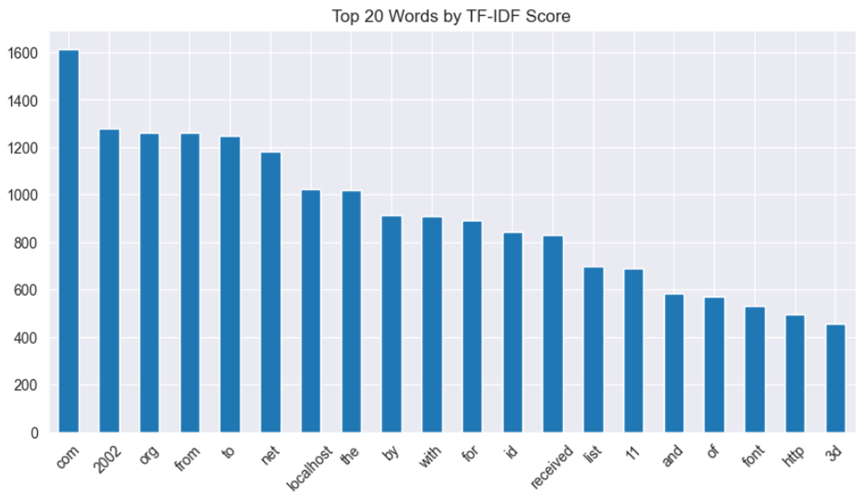
\includegraphics[width=\linewidth]{images/top_tf_idf_score}
    \caption{Bar Chart for Top 20 Words by TF-IDF Score}
    \label{fig:top_tf_idf_score}
\end{figure}

Observations:
\begin{itemize}
    \item ``com'' has the highest TF-IDF score: The word ``com'' has the tallest bar, indicating it has the highest TF-IDF score among the top 20.
    \item ``2002'' and ``org'' have the next highest scores: These words also have relatively high TF-IDF scores.
    \item Words like ``from'', ``to'', ``net'', and ``localhost'' have considerable scores: They suggest some importance in differentiating documents within the corpus.
    \item Common English words have lower scores: Words like ``the'', ``by'', ``with'', ``for'', ``and'', and ``of'' appear in the list but have lower TF-IDF scores compared to the more specific terms.
    This is expected because TF-IDF downweights words that appear frequently across many documents.
    \item Technical terms and identifiers are present: Words like ``id'', ``font'', ``http'', and ``3d'' suggest that these terms might be important in distinguishing certain types of documents within the corpus.
    \item ``received'' and ``list'' also have moderate TF-IDF scores.
    The number ``11'' also appears in the list.
\end{itemize}

Meaning of TF-IDF:
\begin{itemize}
    \item Term Frequency (TF): Measures how frequently a term appears in a document.
    \item Inverse Document Frequency (IDF): Measures how rare a term is across the entire corpus of documents.
    Words that appear in many documents have a lower IDF.
\end{itemize}

A high TF-IDF score for a word means that the word is frequent in a particular document but rare in the overall corpus.
Therefore, these words are considered more important for distinguishing documents.

In summary, this bar chart highlights the words that are most discriminative across the analyzed text documents based on their TF-IDF scores.
The words with higher scores, such as ``com'', ``2002'', ``org'', and ``localhost'', are likely good indicators of the specific content or categories of the documents in which they appear.
The presence of common English words with lower scores confirms the TF-IDF mechanism of prioritizing distinguishing terms.
This analysis is often used in information retrieval and text mining to identify the most relevant terms in a collection of documents.